\section{Implementation}
\label{implementation}

When implementing this mobile application, the following technologies are being used:

\begin{itemize}
  \item \textbf{Flutter 2.2.1} \cite{Flutter}: Flutter is an open-source UI software development kit created by Google. It is used to develop cross platform applications and the web from a single codebase. Flutter was used instead of previously settled technologies such as Java \cite{Java}, Swift \cite{Swift} or Kotlin \cite{Kotlin} due to the first funtional requirement: cross platform compatibility.
  \item \textbf{Android Studio 4.2} \cite{AndroidStudio}: Android Studio is the official integrated development environment (IDE) for Google's Android \cite{Android} operating system. Android Studio is used due to the great compatibility with Flutter.
  \item \textbf{Python 3.8.5} \cite{Python}: Python is an interpreted high-level general-purpose programming language. Python is used due to its community and wide documentation about iamge and video documentation.
  \begin{itemize}
    \item \textbf{Flask 2.0.1} \cite{Flask}: Flask is a micro web framework written in Python. Flask is used due to its ease of use to create APIs. This API is used to integrate the application and Python code.
    \item \textbf{Gunicorn 20.1.0} \cite{Gunicorn}: Gunicorn is a Python WSGI HTTP Server for UNIX. It is used to deploy the API.
    \item \textbf{sqlalchemy 1.4.20} \cite{sqlalchemy}: SQLAlchemy is the Python SQL toolkit and Object Relational Mapper. It is used to design and manage the database.
    \item \textbf{psycopg2 2.9.1} \cite{psycopg2}: Psycopg is the most popular PostgreSQL database adapter for the Python programming language.
  \end{itemize}
  \item \textbf{PostgreSQL 12.7} \cite{postgres}: PostgreSQL is a powerful, open source object-relational database. It is the chosen database to store the data from the analyzed tests and clues.
  \item \textbf{Docker 20.10.7} \cite{Docker}: Docker is a set of platform as a service (PaaS) products that use OS-level virtualization to deliver software in packages called containers. Docker is used due to its portability and scalability.
  \item \textbf{pgAdmin 5.4} \cite{pgAdmin}: pgAdmin is the most popular and feature rich Open Source administration and development platform for PostgreSQL, the most advanced Open Source database in the world.
\end{itemize}

When integrating Python and Flutter, two Flutter plugins were considered:

\begin{itemize}
  \item \textbf{starflut} \cite{starflut}: This plugin was discarded due to the lack of good documentation, since this would make development, maintenance and addition of functionality difficult.
  \item \textbf{chaquopy} \cite{chaquopy}: This plugin is only available for Android \cite{Android}, discarding it with no further research due to the first funtional requirement: cross platform compatibility.
\end{itemize}
\subsection{Mobile application}

For the implementation of the application, four different views have been developed: an info page, a camera preview page, a video preview page and a result page. All of these base pages are parents to the different application screens. This avoids repeating code for similar views. Figure \ref{startpage} shows the Start Page of the application.

\begin{figure}[H]
  \centering
  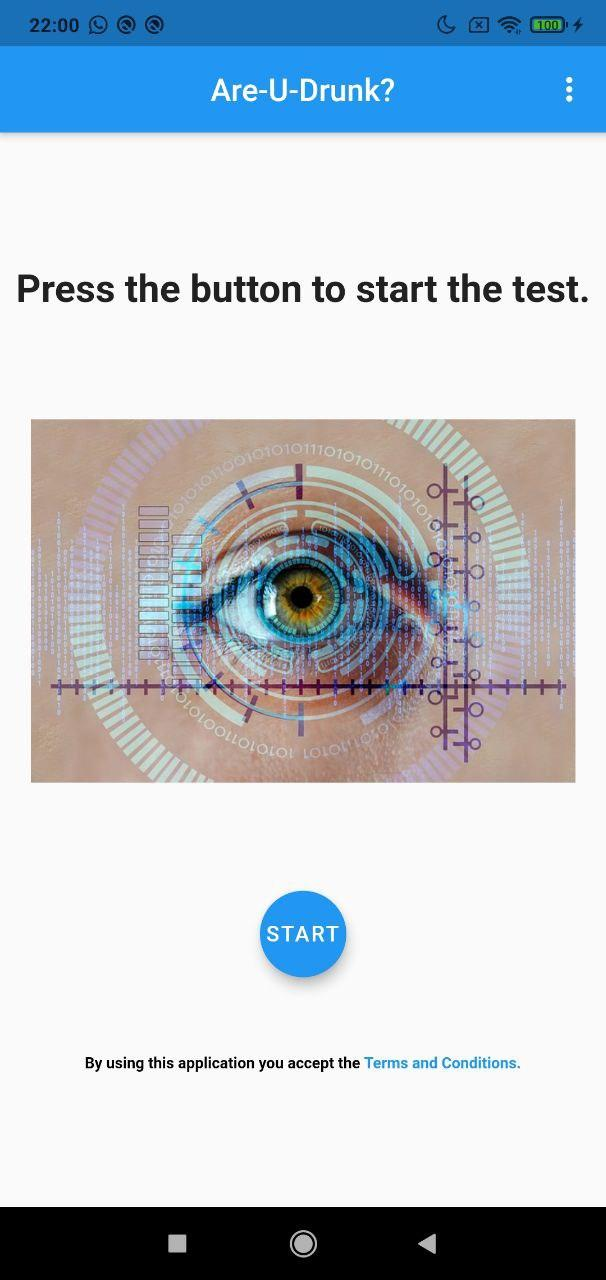
\includegraphics[width=0.25\textwidth]{./img/startpage.jpg}
  \caption{Start Page}
  \label{startpage}
\end{figure}

Code listing \ref{popupcode} shows how the Popup menu button works and listing \ref{termsandconds} how the link to the Terms and Conditions document is created. Listing \ref{startbutton} shows how the button is created and how it calls the backend to initialize the test and the first clue when it is pressed.


\begin{lstlisting}[language=flutter, basicstyle=\small, caption={Popup menu button code}, captionpos=b, label={popupcode}]
PopupMenuButton(
              itemBuilder: (BuildContext bc) => [
                PopupMenuItem(child: Text("Help"), value: "/help"),
              ],
              onSelected: (route) {
                Navigator.push(
                    context,
                    MaterialPageRoute(
                    builder: (context) => HelpPage()));
              },
            )
\end{lstlisting}


\begin{lstlisting}[language=flutter, basicstyle=\small, caption={Terms and Conditions document link}, captionpos=b, label={termsandconds}]
RichText(
  text: new TextSpan(
    children:[
     new TextSpan(
       text:"By using this application you accept the ",
       style: TextStyle(color: Colors.black, fontSize: 10, fontWeight: FontWeight.bold),
     ),
      TextSpan(
        text: "Terms and Conditions.",
        style: new TextStyle(color: Colors.blue, fontSize: 10,fontWeight: FontWeight.bold),
        recognizer: new TapGestureRecognizer()
        ..onTap = () async {
          final url = '<TCs URL>';
          if (await canLaunch(url)) {
            await launch(url, forceSafariVC: false, forceWebView: false);
          }
        },
      )
    ]
  )
)
\end{lstlisting}

\begin{lstlisting}[language=flutter, basicstyle=\small, label={startbutton}, caption={Code to call backend to initialize test and first clue}, captionpos=b]
FloatingActionButton(
                  child: Text("START"),
                  onPressed: () async {
                    await initializeTest();
                    Navigator.push(
                      context,
                      MaterialPageRoute(
                          builder: (context) =>
                              CheckSmoothPursuitLeftPage()),
                    );
                  },
                ),
...
Future<void> initializeTest() async {
    int fatherId = await initialize();
    SharedPreferences prefs = await SharedPreferences.getInstance();
    await prefs.setInt('fatherId', fatherId);
  }
\end{lstlisting}



The calls to the backend are shown in code listings \ref{initialize} and \ref{backendcall}, to call the endpoint to initialize the test and the first clue, and to call an enpoint to proccess each of the clues, respectively. Both calls to the endpoints are done through HTTPS requests.

\begin{lstlisting}[language=flutter, basicstyle=\small, label={initialize}, caption={Code to call the initialize endpoint}, captionpos=b]
Future<int> initialize() async{
  String identifier;
  try {
    identifier = (await UniqueIdentifier.serial)!;
  } on PlatformException {
    identifier = 'Failed to get Unique Identifier';
  }
  Uri url = Uri.https(uri, path + "initialize");
  http.MultipartRequest request =
  new http.MultipartRequest("POST", url);
  request.fields['user'] = identifier;
  http.StreamedResponse response = await request.send();
  final body = await response.stream.bytesToString();
  final responseJson = jsonDecode(body);
  return responseJson['father_id'];
}
\end{lstlisting}

\begin{lstlisting}[language=flutter, basicstyle=\small, label={backendcall}, caption={Code to call the endpoints to proccess each of the clues}, captionpos=b]
Future<String> callBackend(String endpoint, XFile file) async{
  String userIdentifier;
  SharedPreferences prefs = await SharedPreferences.getInstance();
  int fatherId = prefs.getInt('fatherId') ?? 0;
  try {
    userIdentifier = (await UniqueIdentifier.serial)!;
  } on PlatformException {
    userIdentifier = 'Failed to get Unique Identifier';
  }
  Uri url = Uri.https(uri, path + endpoint);
  http.MultipartRequest request =
  new http.MultipartRequest("POST", url);
  http.MultipartFile multipartFile = http.MultipartFile.fromBytes(
      'media', await file.readAsBytes(),
      filename: file.path);
  request.fields['user'] = userIdentifier;
  request.fields['father_test_id'] = fatherId.toString();
  request.files.add(multipartFile);
  http.StreamedResponse response = await request.send();
  final body = await response.stream.bytesToString();
  final responseJson = jsonDecode(body);
  return responseJson['result'];
}
\end{lstlisting}

Figure \ref{clueinfo} shows the page with information about the first clue. It shows a text and a GIF image explaining how to perform the text. Each of the clue has a similar info page.

\begin{figure}[H]
  \centering
  \begin{subfigure}{0.33\textwidth}
      \centering
      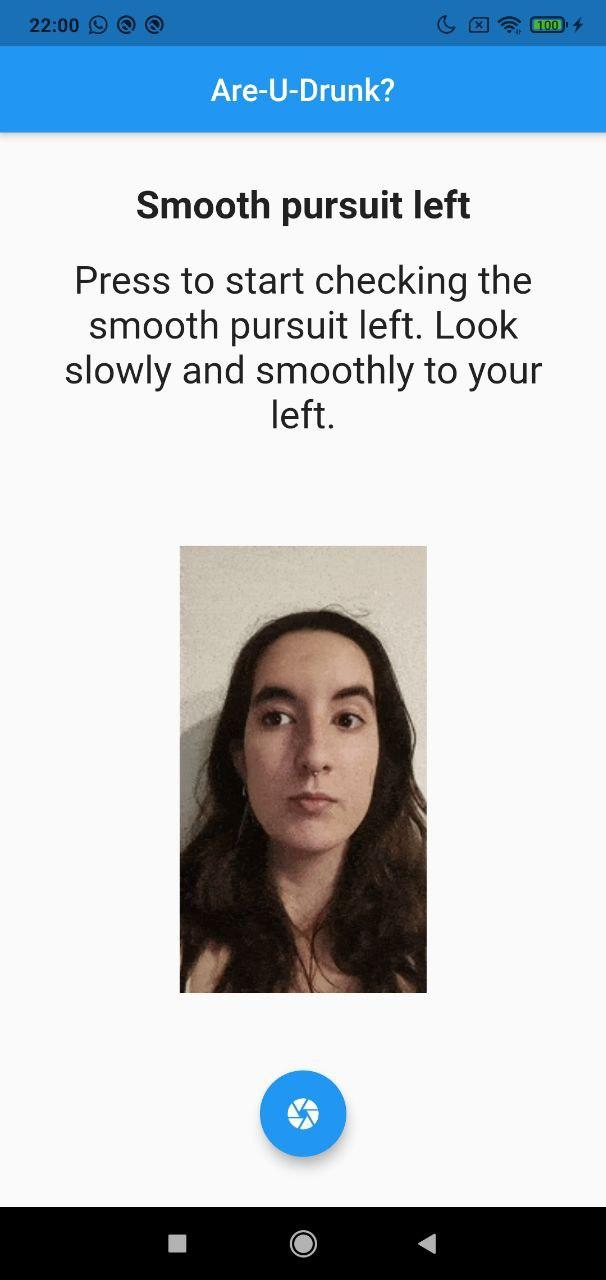
\includegraphics[width=0.5\textwidth]{./img/clueinfo.jpg}
      \caption{Page with information.}
      \label{clueinfo}
  \end{subfigure}\hfill
  \begin{subfigure}{0.33\textwidth}
      \centering
      
\includegraphics[width=0.5\textwidth]{./img/recordvideo.jpg}
      \caption{Page to record the video.}
      \label{recordvideo}
  \end{subfigure}
  \begin{subfigure}{0.33\textwidth}
      \centering
      
\includegraphics[width=0.5\textwidth]{./img/videopreview.jpg}
      \caption{Page to confirm video.}
      \label{videopreview}
  \end{subfigure}
\end{figure}

Code listing \ref{recordvideo} shows the page to record a clue. The user clicks the button to record and the phone starts recording and automatically stops after four seconds and redirects the user to the video preview screen, shown in listing \ref{videopreview}. Listing \ref{recording} shows the code to record the video and stop it automatically, and code listing \ref{preview} shows the call to the backend when the video is confirmed and the code to show a loading animation while the backend is proccessing the request.

\begin{lstlisting}[language=flutter, basicstyle=\small, label={recording}, caption={Code to record video automatically}, captionpos=b]
await _initializeControllerFuture;
await _controller.startVideoRecording();
await Future.delayed(const Duration(seconds: 4), () {});
final image = await _controller.stopVideoRecording();
await Navigator.of(context).push(
MaterialPageRoute(builder: (context) => getNextPage(image.path)));
\end{lstlisting}

\begin{lstlisting}[language=flutter, basicstyle=\small, label={preview}, caption={Code to preview the recorded video}, captionpos=b]
context.loaderOverlay.show();
XFile video = XFile(widget.path);
String result = await callBackend(widget.endpoint, video);
context.loaderOverlay.hide();
\end{lstlisting}


The management of the response is shown in code listing \ref{management}.

\begin{lstlisting}[language=flutter, basicstyle=\small, label={management}, caption={Code to manage the response of the backend}, captionpos=b]
if (result == "fail") {
  failedClues += 1;
}

if (result == "undetected") {
  await Navigator.of(context).push(
    MaterialPageRoute(
        builder: (context) => EyeDetectionFailPage()),
  );
} else {
  if (failedClues < 2) {
    // If the picture was taken, display it on a new screen.
    await Navigator.of(context).push(
      MaterialPageRoute(
          builder: (context) => widget.getNextPage()),
    );
  } else {
    failedClues = 0;
    await Navigator.of(context).push(
      MaterialPageRoute(
          builder: (context) => DrunkPage()),
    );
  }
}
\end{lstlisting}
When the final result is obtained (eyes not detected, fail or pass), a similar screen to figure \ref{finalresult} is shown.

\begin{figure}[H]
  \centering
  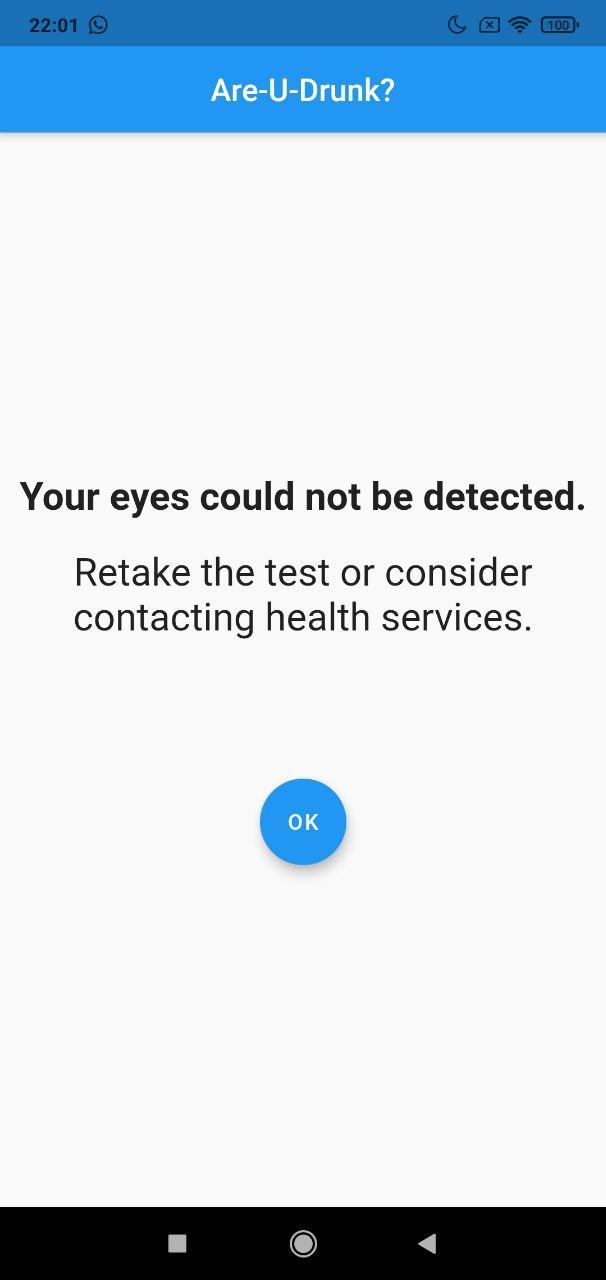
\includegraphics[width=0.22\textwidth]{./img/finalresult.jpg}
  \caption{Eyes not detected screen}
  \label{finalresult}
\end{figure}

\subsection{Server}

The server side uses Docker to host both the database and API. The interaction between the API and the database can be seen in Figure \ref{architecture}. This server is composed by an Application Programming Interface developed with Python and Gunicorn to receive data from the smartphone application and query the database, and a PostgreSQL database to store the videos recorded by de application. As previously mentioned, sqlalchemy is the toolkit used to query the database from the API.

Code listing \ref{docker-compose} shows the docker-compose.

\begin{lstlisting}[language=docker-compose-2, label={docker-compose}, caption={docker-compose}, captionpos=b]
version: '3'
services:
  database:
    image: "postgres:9.6.22-buster" # use 9.6.22-buster postgres version
    env_file:
      - database.env # configure postgres
    volumes:
      - database-data:/var/lib/postgresql/data/ # persist data even if container shuts down
    ports:
      - "60123:5432"
  backend:
    image: are_u_drunk_rest_api
    build: .
    ports:
      - "60321:5000"
    volumes:
      - clue-videos:/app/videos
volumes:
  database-data:
  clue-videos:
\end{lstlisting}

With this docker-compose, the database and backend services are created. The database service uses a volume to persist the data inserted when the service stops and starts again. The backend service uses a volume to store the videos recorded by the application and referenced in the database entries.


\begin{lstlisting}[language=docker, label={dockerfile}, caption={Dockerfile}, captionpos=b]
FROM python:3.8.11-slim-buster
RUN apt-get update && apt-get install -y libpq-dev gcc python3-dev musl-dev g++ libglib2.0-dev python3-opencv libopencv-dev
COPY requirements.txt /
RUN pip3 install -r /requirements.txt
RUN pip3 install ipython
COPY ./src /app
COPY ./run.sh /app
COPY ./gunicorn.conf.py /app
WORKDIR /app
ENV PYTHONPATH /app
RUN mkdir videos
ENTRYPOINT ["./run.sh"]
\end{lstlisting}

Code listing \ref{dockerfile} shows how the container is instantiated: a Python Docker image is used, the dependencies and requirements are installed, and finally, the code is copied to the container's root and \textit{run.sh} is set as the entry point. \textit{run.sh} initializes the app with the specified configuration in the Gunicorn config file. Also a directory named "videos" is created to store the videos recorded by the application.

As previously mentioned, Docker is used due to its ease to scale and deploy, and using the command shown in Figure \ref{dockercommand} the API and the backend can be set up in the environment (development and production).

\begin{lstlisting}[language=bash, mathescape=false, label={dockercommand}, caption={Commands to set the environment up}, captionpos=b]
$> docker-compose up --build d
\end{lstlisting}

\subsubsection{Database}

The database has been implemented following the schema shown in figure \ref{databaseschema}.

\begin{figure}[H]
    \centering
    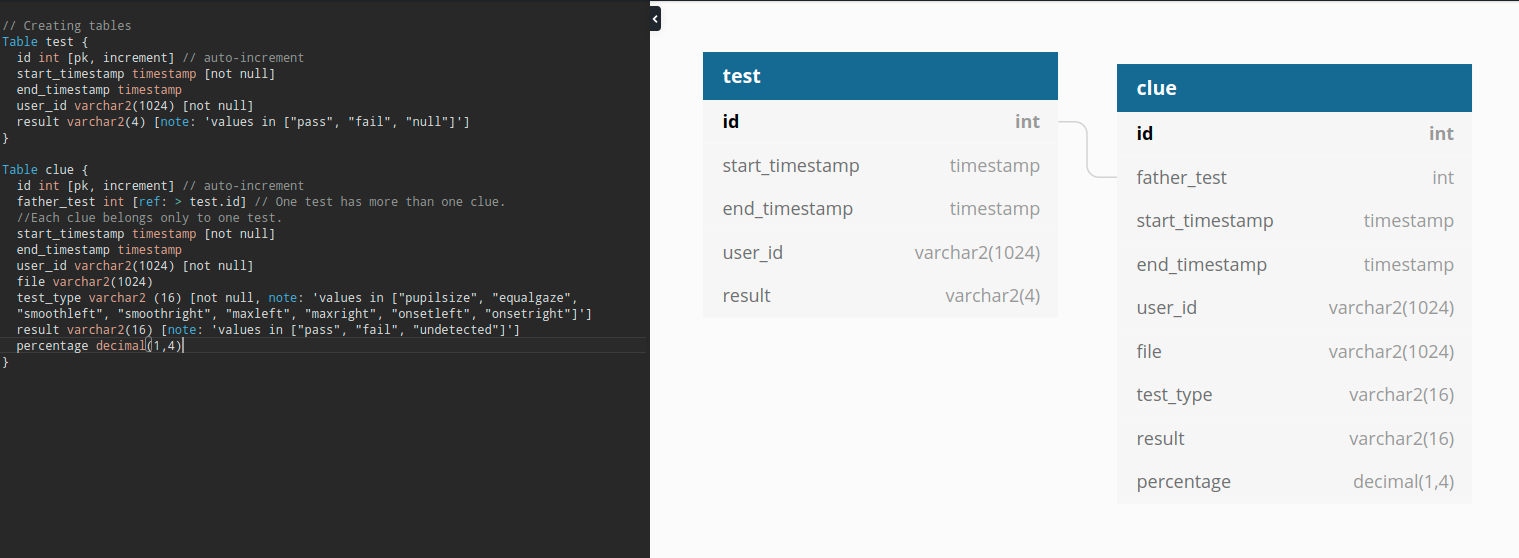
\includegraphics[width=0.95\textwidth]{./img/db.png}
    \caption{Database schema}
    \label{databaseschema}
\end{figure}

The entity \textit{Test} has an id (auto-incremental), a start timestamp (not nullable), an end timestamp (nullable), an unique identifier of the user who took the test (not nullable) and the result (nullable). The start timestamp is inserted as soon as the test begins and the end timestamp is updated as soon as the user ends each of the clue, so we could be able to trace if the user quits before ending the test and where. The result is inserted when the user finishes the last clue, either the 6th clue, the second failed clue or one in which the eyes are not recognized. With this implementation, if the user doesn't finish the test, the result is null and we could query the end timestamp to know in which clue the user quitted.

The entity \textit{Clue} has an id (auto-incremental), the id of the father test (not nullable), a start timestamp (not nullable), an end timestamp (nullable), an unique identifier of the user who took the test (not nullable), the path to the video file (nullable), the test type (not nullable), the result (nullable) and the percentage of success. The start timestamp is inserted as soon as the clue begins and the end timestamp is updated as soon as the user ends each of the clue, so we could be able to trace if the user quits while taking that clue. Therefore, the video file path is nullable since the user could quit and no video would be recorded. The result is inserted when the user finishes the clue. With this implementation, we could query either the result or the end timestamp to know if the user finished the clue.

\subsubsection{Python API}

The API consists of two classes to integrate with the database, seven different endpoints and seven different methods to analyze the video. The model definition for 'Clue' entity is shown in figure \ref{cluepy}.

  \begin{python}[basicstyle=\small, label={cluepy}, caption={Clue class in clue.py}, captionpos=b]
    class Clue(Base):
        __tablename__ = 'clue'
        id = Column(Integer, primary_key=True)
        father_test = Column(Integer, ForeignKey('test.id'))
        start_timestamp = Column(DateTime, nullable=False)
        end_timestamp = Column(DateTime, nullable=True)
        user_id = Column(String, nullable=False)
        file = Column(String, nullable=True)
        test_type = Column(String, nullable=False)
        result = Column(String, nullable=True)
        def __init__(self, father_test, start_timestamp, end_timestamp, user_id, file, test_type, result):
            self.father_test = father_test
            self.start_timestamp = start_timestamp
            self.end_timestamp = end_timestamp
            self.user_id = user_id
            self.file = file
            self.test_type = test_type
            self.result = result
  \end{python}

Out of the seven different endpoints, one is to initialize the test and the first clue and the six remaining are called when a clue ends. Figure \ref{maximumright} shows the endpoint called when the maximum deviation right is checked.

\begin{python}[label={maximumright}, caption={Enpoint to proccess the maximum deviation right}, captionpos=b]
  @app.route('/maximumright', methods=['POST'])
  def maximum_right():
    user = request.form['user']
    father_test_id = int(request.form['father_test_id'])
    time = datetime.utcnow()
    filename=f"{user}-{time.strftime('\%Y-\%m-\%d \%H:\%M:\%S')}-maximumright.mp4"
    request.files['media'].save(filename)
    perc = get_percentage(filename, 'right')
    if perc > LIMIT:
        return_result = "pass"
    elif perc == 0:
        return_result = "undetected"
    else:
        return_result = "fail"
    _insert_into_db(father_test_id=father_test_id, return_result=return_result, user=user, filename=filename,
                    current_clue_type="maximumright", time=time, percentage=perc)
    return {'result': return_result}
\end{python}

The six endpoints to proccess the clues follow the same structure: the request parameters are obtained (user who called the backend, the id assigned to the test that groups all the clues and the video recorded) and the video is saved, naming it after the user, the timestamp of the call and the type of clue. Then, the method to track and analyze the gaze and determine whether the clue is passed or not and depending on the result, the corresponding operations are performed in the database. Finally, the result is sent as a response. Figure \ref{getpercentage} shows the method previously mentioned. This code is based on Proctoring-AI project \cite{proctoringai}.


  \begin{python}[basicstyle=\footnotesize, caption={Method to track and analyze the gaze and determine whether the clue is passed or not}, captionpos=b, label={getpercentage}]
    def get_percentage(video, gaze):
    try:
        left_data_list = []
        right_data_list = []
        face_model = get_face_detector()
        landmark_model = get_landmark_model()
        left = [36, 37, 38, 39, 40, 41]
        right = [42, 43, 44, 45, 46, 47]
        cap = cv2.VideoCapture(video)
        kernel = np.ones((9, 9), np.uint8)
        while cap.isOpened():
            ret, img = cap.read()
            if ret:
                rects = find_faces(img, face_model)

                for rect in rects:
                    try:
                        shape = detect_marks(img, landmark_model, rect)
                    except cv2.error:
                        continue
                    mask = np.zeros(img.shape[:2], dtype=np.uint8)
                    mask, end_points_left = eye_on_mask(mask, left, shape)
                    mask, end_points_right = eye_on_mask(mask, right, shape)
                    mask = cv2.dilate(mask, kernel, 5)
                    eyes = cv2.bitwise_and(img, img, mask=mask)
                    mask = (eyes == [0, 0, 0]).all(axis=2)
                    eyes[mask] = [255, 255, 255]
                    mid = int((shape[42][0] + shape[39][0]) // 2)
                    eyes_gray = cv2.cvtColor(eyes, cv2.COLOR_BGR2GRAY)
                    threshold = 75
                    _, thresh = cv2.threshold(eyes_gray, threshold, 255, cv2.THRESH_BINARY)
                    thresh = process_thresh(thresh)
                    contouring(thresh[:, 0:mid], mid, img, end_points_left, False, right_data_list, left_data_list)
                    contouring(thresh[:, mid:], mid, img, end_points_right, True, right_data_list, left_data_list)
                    for (x, y) in shape[36:48]:
                        cv2.circle(img, (x, y), 2, (255, 0, 0), -1)
            else:
                break
        cap.release()
        cv2.destroyAllWindows()
        try:
            if gaze == 'right':
                result = count_wrong_meassurements(right_data_list, True) / len(right_data_list)
            else:
                 result = count_wrong_meassurements(left_data_list) / len(left_data_list)
            return 1 - result
        except ZeroDivisionError:
            return 0
    except cv2.error:
        logger.exception("Exception detecting eyes")
        return 0
  \end{python}

In the get\_percentage method, two arrays are firstly created to store the points obtained from the eyes, the face detector and landmark model are instantiated and the landmark coordinates for the left and right eyes are harcoded. These landmark coordinates are obtained from the Dlib facial keypoints. Then, the video is analyzed frame by frame, detecting firstly the eyes with the eye\_on\_mask method and then detecting the eye position with the contouring method. All of the positions are stored in the corresponding data list and when the video is completely analyzed, the percentage of positions that are invalid is calculated. A position is considered invalid when the previous one is greater in the case of a left gaze and smaller in the case of a right gaze. If no data is stored in the list, eyes have not been detected and the method returns zero.

\subsubsection{Deployment}

This project has been uploaded to a server provided by de University of Granada \cite{ugr}. For this purpose, the requests have been proxied through Nginx \cite{nginx}. This is also useful to isolate the Are-U-Drunk project from the rest of the projects hosted in the server. To deploy the system, Docker is required in the server. Once this requirement is met, the application has to be downloaded from the repository and copied to the server. Then, the Gunicorn config file has to be modified to set the new path for the requests and using the command shown in listing \ref{dockercomposeup} the containers for the services start working.

\begin{lstlisting}[label={dockercomposeup}, caption={Command to start the containers}, captionpos=b]
docker-compose up
\end{lstlisting}

The database is created by means of two scripts, one for each table. Listing \ref{dbscript} shows the script used to create the table for the tests. A database.env file has to be created to configure secure credentials to access the database.

\begin{lstlisting}[label={dbscript}, caption={Script to create the table for the tests}, captionpos=b]
SET statement_timeout = 0;
SET lock_timeout = 0;
SET idle_in_transaction_session_timeout = 0;
SET client_encoding = 'UTF8';
SET standard_conforming_strings = on;
SELECT pg_catalog.set_config('search_path', '', false);
SET check_function_bodies = false;
SET xmloption = content;
SET client_min_messages = warning;
SET row_security = off;
SET default_tablespace = '';
CREATE TABLE public.test (
    id integer NOT NULL,
    start_timestamp timestamp without time zone NOT NULL,
    end_timestamp timestamp without time zone,
    user_id character varying NOT NULL,
    result character varying
);
ALTER TABLE public.test OWNER TO cdg;
CREATE SEQUENCE public.test_id_seq
    START WITH 1
    INCREMENT BY 1
    NO MINVALUE
    NO MAXVALUE
    CACHE 1;
ALTER TABLE public.test_id_seq OWNER TO cdg;
ALTER SEQUENCE public.test_id_seq OWNED BY public.test.id;
ALTER TABLE ONLY public.test ALTER COLUMN id SET DEFAULT nextval('public.test_id_seq'::regclass);
ALTER TABLE ONLY public.test
    ADD CONSTRAINT test_pkey PRIMARY KEY (id);
\end{lstlisting}

Finally, the path to the application is added to nginx to redirect the request and the service is restarted. Listing \ref{nginxcode} shows this change.

\begin{lstlisting}[label={nginxcode}, caption={Nginx configuration file}, captionpos=b, mathescape]
server {
	listen 80 default_server;
	listen [::]:80 default_server;
	server_name _;
	return 301 https://hostrequest_uri;

}

server {
	listen 443 ssl default_server;
	listen [::]:443 ssl default_server;
	...
  location /are_u_drunk_backend {
    proxy_pass  http://localhost:60321;
    proxy_set_header Host host;
    proxy_set_header X-Real-IP remote_addr;
    proxy_set_header X-Forwarded-For proxy_add_x_forwarded_for;
	}
  ...
}
\end{lstlisting}
